%%%%%%%%%%%%%%%%%%%%%%%%%%%%%%%%%%%%%%%%%%%%%%%%%%%%%%%%%%
%%
%% MARK: Title & Data
%%
%%%%%%%%%%%%%%%%%%%%%%%%%%%%%%%%%%%%%%%%%%%%%%%%%%%%%%%%%%

\chapter*{\sf Seifert Orbifolds}
\setcounter{footnote}{0}

%%%%%%%%%%%%%%%%%%%%%%%%%%%%%%%%%%%%%%%%%%%%%%%%%%%%%%%%%%
%%
%% MARK: Abstract
%%
%%%%%%%%%%%%%%%%%%%%%%%%%%%%%%%%%%%%%%%%%%%%%%%%%%%%%%%%%%

\begin{abstract}
  The quotient of a $3$-manifold by an effective action of $\Sph^1$,
  without fixed points,
  is a classical example of an orbifold.
  But how does this fit within the diffeological framework?%
  %That is what we discuss here.%
  %\footnote{This is a joint note with Jean-Paul Mohsen.}
\end{abstract}

%%%%%%%%%%%%%%%%%%%%%%%%%%%%%%%%%%%%%%%%%%%%%%%%%%%%%%%%%%
%%
%% MARK: Content
%%
%%%%%%%%%%%%%%%%%%%%%%%%%%%%%%%%%%%%%%%%%%%%%%%%%%%%%%%%%%

We will discuss classical constructions in differential geometry,
but from the point of view of diffeology.
We will see how,
in this example,
the vocabulary and constructions of diffeology fit the needs of the problem.
We shall consider in particular the diffeological definition of an orbifold,
that is,
a diffeological space locally diffeomorphic to a quotient $\RR^n/\Gamma$,
where $\Gamma$ is a finite subgroup of the linear group $\GL(n,\RR)$,
see \cite{IKZ10} for the details.

\textbf{Warning.} One should not confuse what we call in this note a "Seifert orbifold" with what topologists call a "Seifert fibered orbifold",
as appears in \cite{BoSi85} for example.
For us the orbifold is the space of Seifert fibers of a Seifert fibered manifold,
and not an orbifold that would be the total space of a Seifert fibration.

%%%%%%%%%%%%%%%%%%%%%%%%%%%%%%%%%%%%%%%%%%%%%%%%%%%%%%%%%%
%%
%% MARK: Smooth Lie Group Actions
%%
%%%%%%%%%%%%%%%%%%%%%%%%%%%%%%%%%%%%%%%%%%%%%%%%%%%%%%%%%%

\section{A little bit of smooth Lie group actions}

Consider a smooth action of a Lie group $G$ on a manifold $M$.

(A) Diffeologically speaking,
such an action is a smooth homomorphism $g \mapsto g_M$,
from $G$ to $\Diff(M)$,
where $\Diff(M)$ is equipped with the functional diffeology \cite[\textsection\,7.4]{PIZ13}.

(B) Let $x \in M$ and let $H = \Stab(x)$ be the stabilizer of $x$.
The orbit map $g \mapsto g_M(x)$ from $G$ to $M$ is strict,
meaning that the projection $\Class(g) \mapsto g_M(x)$,
defined on the coset $G/H$ into $M$, is an induction.
In other words,
the map $\Class: G/H \to \cO_x$ is a diffeomorphism,
where $G/H$ is equipped with the quotient diffeology and $\cO_x \subset M$ is equipped with the subset diffeology \cite[\textsection\,1]{IZK12}:
equipped with the subset diffeology,
the orbit $\cO_x$ is a manifold diffeomorphic to the coset $G/H$.
Now,
if $G$ is compact,
then this induction is an embedding and the orbit is an embedded submanifold.

(C) If $G$ is compact,
the type of stabilizers (or orbits) of a smooth action of $G$ on a manifold $M$
is given by the \emph{Theorem of Principal Orbits} \cite[Theorem 3.1 of Part IV]{Bre72}.

\begin{Article}{Principal orbits.}{}
  There exists a maximal orbit type $G/H$ for $G$ on $M$
  (i.e., $H$ is conjugate to a subgroup of every isotropy group).
  The union $M_{(H)}$ of the orbits of type $G/H$ is open and dense in $M$.
  
  In particular,
  the stabilizers of any two points in $M_{(H)}$ are conjugate.
  The orbits of points in $M_{(H)}$ are called \emph{principal orbits}.
\end{Article}

Non-principal orbits are called \emph{singular orbits}.
If a singular orbit has the same dimension as the principal orbits,
the orbit is said to be \emph{exceptional}.

(D) If $G$ is compact,
Theorem 2.4 of Part VI of \emph{Compact Group Actions on Manifolds} \cite{Bre72} states that:

\begin{Article}{Smooth linear tube.}{}
  Let $x$ be any point in $M$,
  and let $H$ be the stabilizer of $x$.
  There exists a vector space $V$,
  an orthogonal action of $H$ on $V$,
  and a local $G$-invariant diffeomorphism $\varphi : G \times_H V \to M$.
\end{Article}

The space $G \times_H V$ is the quotient of $G \times V$ by the diagonal action of $H$:
$h_{G \times V}: (g,v) \mapsto (gh^{-1}, h_V(v))$,
where $h \mapsto h_V$ denotes the action of $H$ on $V$.

The image of the local diffeomorphism $\varphi$ is an open invariant tube about the orbit $\cO_x$,
the image under $\varphi$ of the zero section in $G \times_H V$.

%%%%%%%%%%%%%%%%%%%%%%%%%%%%%%%%%%%%%%%%%%%%%%%%%%%%%%%%%%
%%
%% MARK: Circle actions on manifolds
%%
%%%%%%%%%%%%%%%%%%%%%%%%%%%%%%%%%%%%%%%%%%%%%%%%%%%%%%%%%%

\section{Circle actions on manifolds}

Consider a smooth action of the circle $\Sph^1$ on a manifold $M$.
According to the Theorem of Principal Orbits for compact group actions on manifolds,
there exists an $\Sph^1$-invariant open dense subset of $M$ such that all of its points have the same principal stabilizer $H$,
a closed subgroup of $\Sph^1$.
Moreover, this principal stabilizer is contained in every stabilizer.

If the principal stabilizer is $\Sph^1$ then all stabilizers are $\Sph^1$ and the action is trivial.

If the action is non-trivial then $H$ is a cyclic group $\ZZ_m = \{\epsilon \mid \epsilon^m = 1\}$.

In the case of a non-trivial action of $\Sph^1$,
it is always possible to consider the quotient group $\Sph^1/H$,
which is isomorphic to $\Sph^1$,
and the situation is reduced to an effective action of $\Sph^1$,
that is,
an action with principal stabilizer $\{1\}$.
This is what we assume from now on.

If the action has no fixed points then the singular orbits are exceptional,
and conversely.

%%%%%%%%%%%%%%%%%%%%%%%%%%%%%%%%%%%%%%%%%%%%%%%%%%%%%%%%%%
%%
%% MARK: Seifert orbifolds
%%
%%%%%%%%%%%%%%%%%%%%%%%%%%%%%%%%%%%%%%%%%%%%%%%%%%%%%%%%%%

\section{Seifert orbifolds}

Now we can present the object of our note.
We refer to \cite{Sco83} for the vocabulary and general context.

\begin{Article}{Seifert fibration.}{\itshape
  A \emph{Seifert fibered space} (or Seifert fibration) is a $3$-manifold $M$ with an effective action of $\Sph^1$ without fixed points.
  }
\end{Article}

Because all the stabilizers are cyclic,
the \emph{fibers} of the Seifert fibered space,
that is,
the orbits of the action of the circle,
are diffeomorphic to the circle
when equipped with their subset diffeology \cite[\textsection\,1]{IZK12}.
What about the quotient space?

\begin{Article}{Seifert orbifolds.}{}
  Let $M$ be a $3$-manifold with an effective action of $\Sph^1$,
  without fixed points.
  Then the quotient space $Q = M/\Sph^1$ is a $2$-manifold if the action is principal,
  or a $2$-orbifold with isolated conic singularities otherwise.
\end{Article}

\begin{proof}
  Thanks to the Linear Tube Theorem,
  every orbit $\cO_x$ has an equivariant open neighborhood diffeomorphic to a linear tube of the form $\Sph^1 \times_{\ZZ_m} \CC$,
  where $\ZZ_m$ is the stabilizer of $x$.
  Then,
  about the orbit $\cO_x \in Q$,
  the quotient space $Q$ is locally diffeomorphic to $(\Sph^1 \times_{\ZZ_m} \CC)/\Sph^1$,
  where the action of $\Sph^1$ is given by $\tau \cdot \Class(z,Z) = \Class(\tau z, Z)$.
  Note in particular that $\Class(z,Z) = z \cdot \Class(1,Z)$.
  
  Consider the map $\J : \CC \to \Sph^1 \times_{\ZZ_m} \CC$,
  defined by $\J(Z) = \Class(1,Z)$.
  The map $\J$ is an induction.
  Indeed,
  it is clearly injective.
  Moreover,
  let $r \mapsto \zeta(r)$ be a plot in $\J(\CC) \subset \Sph^1 \times_{\ZZ_m} \CC$.
  Since $\Class : \Sph^1 \times \CC \to \Sph^1 \times_{\ZZ_m} \CC$ is a subduction by construction,
  there exist plots $r \mapsto (z(r), Z(r))$ in $\Sph^1 \times \CC$ such that,
  locally,
  $\zeta(r) = \Class(z(r), Z(r))$.
  But since $\zeta(r) \in \J(\CC)$,
  for every $r$ in the domain of the plot there exists $Z' \in \CC$ such that $\Class(z(r), Z(r)) = \Class(1, Z')$.
  Thus $z(r) \in \ZZ_m \subset \Sph^1$,
  and since $\ZZ_m \subset \Sph^1$ is diffeologically discrete,
  $r \mapsto z(r)$ is locally constant,
  so $z(r) = \epsilon \in \ZZ_m$.
  Hence,
  $\zeta(r) =_{\text{loc}} \Class(1, \epsilon Z(r))$,
  with $r \mapsto \epsilon Z(r)$ smooth.
  Therefore,
  $\J$ is an induction.
  
  Next,
  every $\Sph^1$-orbit in $\Sph^1 \times_{\ZZ_m} \CC$ writes $\Sph^1 \cdot \Class(1,Z) = \{\Class(z,Z) \mid z \in \Sph^1\}$,
  for some $Z \in \CC$.
  Its intersection with $\J(\CC)$ is the set
  $$%
    \big(\Sph^1 \cdot \Class(1,Z)\big) \cap \J(\CC) = \{\Class(1,\epsilon Z) = \J(\epsilon Z) \mid \epsilon \in \ZZ_m\}.
    $$%
  Thus,
  there exists a natural bijection $j : \CC/\ZZ_m \to (\Sph^1 \times_{\ZZ_m} \CC)/\Sph^1$ mapping each $\ZZ_m$-orbit in $\CC$ to the corresponding $\Sph^1$-orbit in $\Sph^1 \times_{\ZZ_m} \CC$:
  $$%
    j(\Class(Z)) = \Sph^1 \cdot \Class(1,Z).
    $$%
  
  Let $\Proj : \Sph^1 \times_{\ZZ_m} \CC \to (\Sph^1 \times_{\ZZ_m} \CC)/\Sph^1$ be the natural projection.
  Let us prove that the restriction $\Proj \restriction \J(\CC)$ is still a subduction.
  Let $r \mapsto \zeta(r)$ be a plot in $(\Sph^1 \times_{\ZZ_m} \CC)/\Sph^1$.
  Locally $\zeta(r) = \Proj(\Class(z(r), Z(r)))$,
  where $r \mapsto z(r)$ and $r \mapsto Z(r)$ are smooth.
  But $\Class(z(r), Z(r)) = z(r) \cdot \Class(1, z(r) Z(r))$,
  so $\Proj(\Class(z(r), Z(r))) = \Proj(\Class(1, z(r) Z(r)))$,
  and $\Class(1, z(r) Z(r))$ belongs to $\J(\CC)$.
  Thus,
  as claimed,
  $\Proj \restriction \J(\CC)$ is still a subduction.
  
  Therefore,
  since $\Class : \CC \to \CC/\ZZ_m$ and $\Proj \restriction \J(\CC) : \J(\CC) \to (\Sph^1 \times_{\ZZ_m} \CC)/\Sph^1$ are subductions,
  since $\J$ is an induction,
  and the factorization $j : \CC/\ZZ_m \to (\Sph^1 \times_{\ZZ_m} \CC)/\Sph^1$ is a bijection,
  $j$ is a diffeomorphism.
  
  $$%
    \begin{tikzcd}
    \CC \arrow{r}{\J} \arrow[swap]{d}{\Class} & \Sph^1 \times_{\ZZ_m} \CC \arrow{d}{\Proj} \arrow{r}{\pphi}       & M  \arrow{d}{\pi} \\
    \CC/\ZZ_m \arrow{r}[swap]{j}                                   & (\Sph^1 \times_{\ZZ_m} \CC)/\Sph^1 \arrow{r}[swap]{f} & M/\Sph^1
    \end{tikzcd}
    $$%
  
  Finally,
  the equivariant local diffeomorphism $\pphi : \Sph^1 \times_{\ZZ_m} \CC \to M$,
  given by the Smooth Linear Tube Theorem above,
  projects onto a local diffeomorphism $f : (\Sph^1 \times_{\ZZ_m} \CC)/\Sph^1 \to M/\Sph^1$.
  The composite $f \circ j$ is then a local diffeomorphism from $\CC/\ZZ_m$ into $M/\Sph^1$.
  Therefore,
  $M/\Sph^1$ is an orbifold according to \cite[Definition 6]{IKZ10}.
  The singular points are the images under $f \circ j$ of $\Class(0) \in \CC/\ZZ_m$.
  They are clearly isolated and conic.
  If there are no exceptional orbits,
  then $M/\Sph^1$ is obviously just a manifold (which is a direct consequence of the Linear Tube Theorem).
\end{proof}

\vfill
\centerline{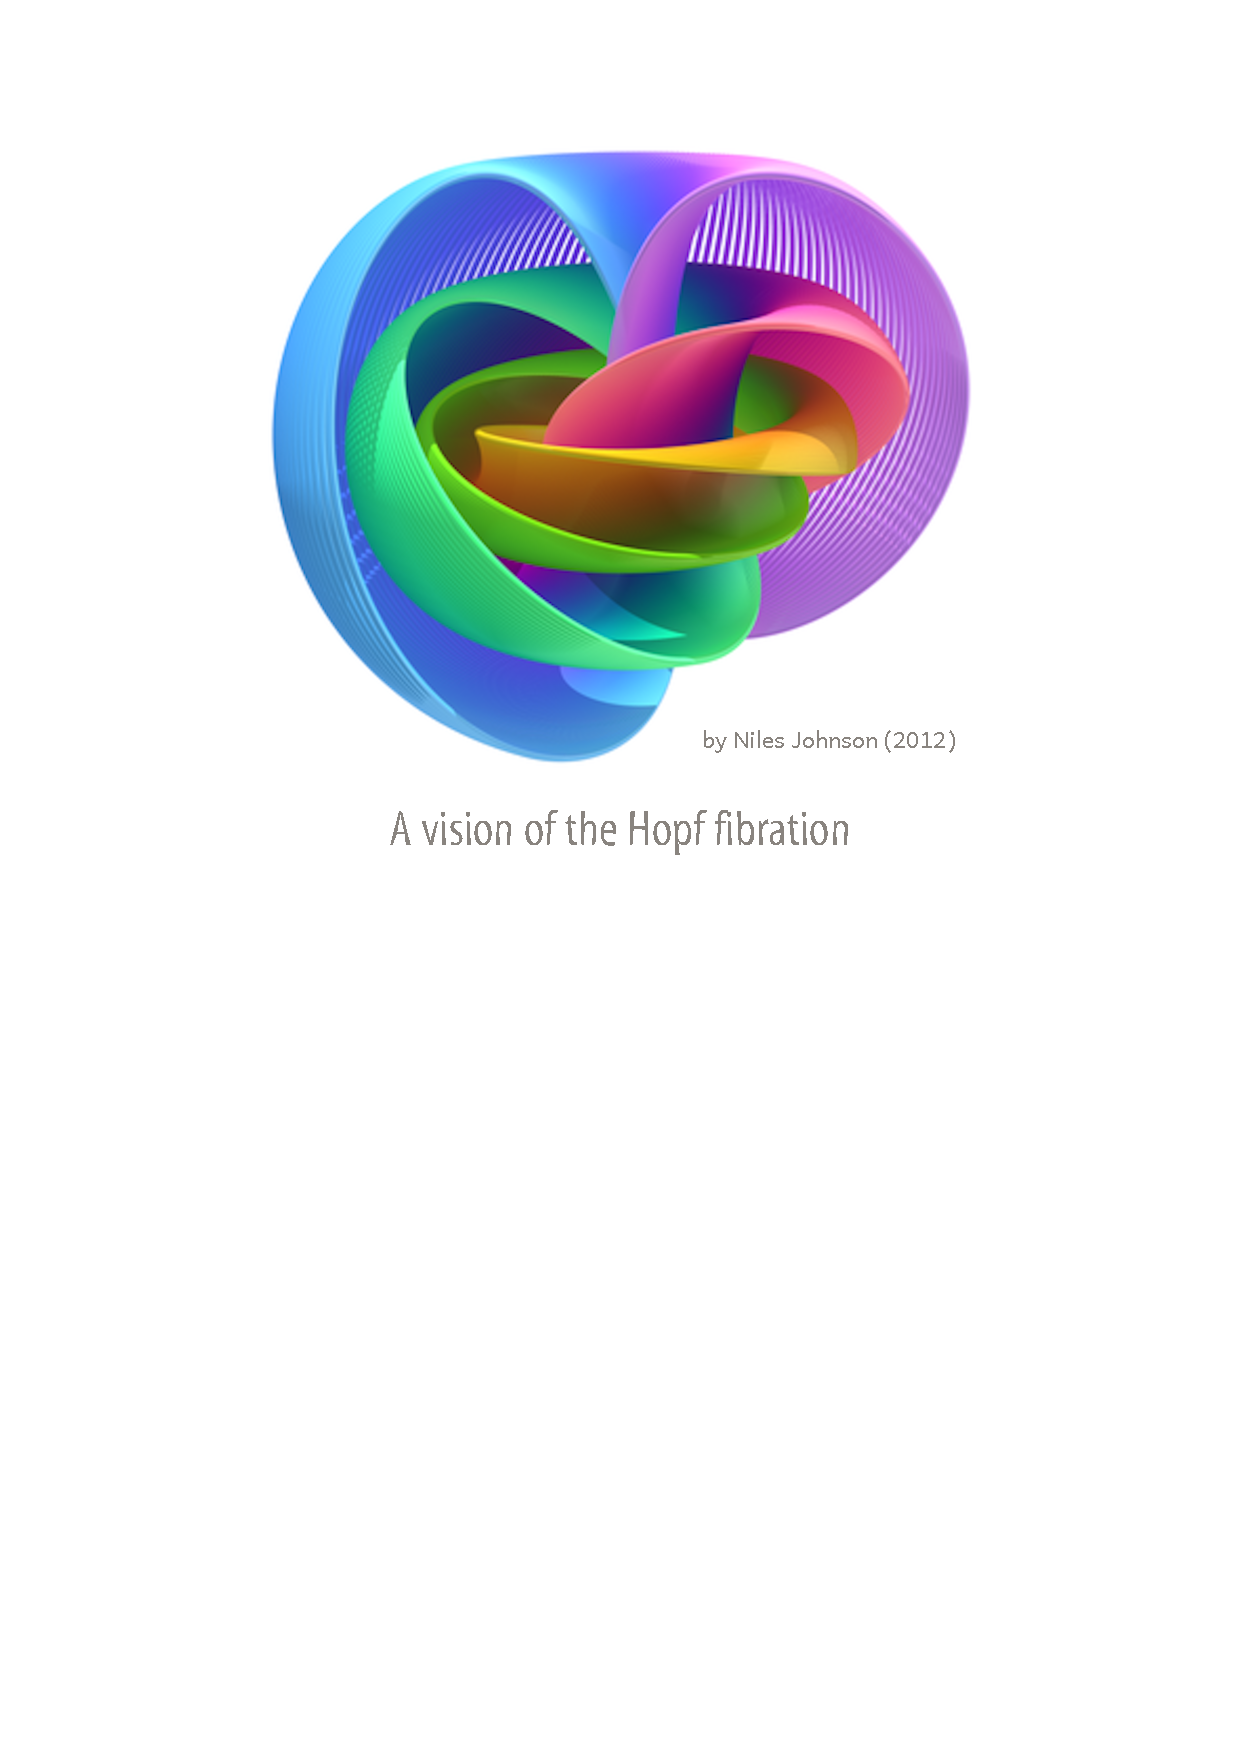
\includegraphics[width=.7\textwidth]{Figures/Hopf.pdf}}
